\documentclass[twoside]{book}

% Packages required by doxygen
\usepackage{calc}
\usepackage{doxygen}
\usepackage{graphicx}
\usepackage[utf8]{inputenc}
\usepackage{makeidx}
\usepackage{multicol}
\usepackage{multirow}
\usepackage{textcomp}
\usepackage[table]{xcolor}

% NLS support packages
\usepackage{hfont}

% Font selection
\usepackage[T1]{fontenc}
\usepackage{mathptmx}
\usepackage[scaled=.90]{helvet}
\usepackage{courier}
\usepackage{amssymb}
\usepackage{sectsty}
\renewcommand{\familydefault}{\sfdefault}
\allsectionsfont{%
  \fontseries{bc}\selectfont%
  \color{darkgray}%
}
\renewcommand{\DoxyLabelFont}{%
  \fontseries{bc}\selectfont%
  \color{darkgray}%
}

% Page & text layout
\usepackage{geometry}
\geometry{%
  a4paper,%
  top=2.5cm,%
  bottom=2.5cm,%
  left=2.5cm,%
  right=2.5cm%
}
\tolerance=750
\hfuzz=15pt
\hbadness=750
\setlength{\emergencystretch}{15pt}
\setlength{\parindent}{0cm}
\setlength{\parskip}{0.2cm}
\makeatletter
\renewcommand{\paragraph}{%
  \@startsection{paragraph}{4}{0ex}{-1.0ex}{1.0ex}{%
    \normalfont\normalsize\bfseries\SS@parafont%
  }%
}
\renewcommand{\subparagraph}{%
  \@startsection{subparagraph}{5}{0ex}{-1.0ex}{1.0ex}{%
    \normalfont\normalsize\bfseries\SS@subparafont%
  }%
}
\makeatother

% Headers & footers
\usepackage{fancyhdr}
\pagestyle{fancyplain}
\fancyhead[LE]{\fancyplain{}{\bfseries\thepage}}
\fancyhead[CE]{\fancyplain{}{}}
\fancyhead[RE]{\fancyplain{}{\bfseries\leftmark}}
\fancyhead[LO]{\fancyplain{}{\bfseries\rightmark}}
\fancyhead[CO]{\fancyplain{}{}}
\fancyhead[RO]{\fancyplain{}{\bfseries\thepage}}
\fancyfoot[LE]{\fancyplain{}{}}
\fancyfoot[CE]{\fancyplain{}{}}
\fancyfoot[RE]{\fancyplain{}{\bfseries\scriptsize Generated on Tue Jun 9 2015 22\-:25\-:26 for C\-O\-S\-S\-B by Doxygen }}
\fancyfoot[LO]{\fancyplain{}{\bfseries\scriptsize Generated on Tue Jun 9 2015 22\-:25\-:26 for C\-O\-S\-S\-B by Doxygen }}
\fancyfoot[CO]{\fancyplain{}{}}
\fancyfoot[RO]{\fancyplain{}{}}
\renewcommand{\footrulewidth}{0.4pt}
\renewcommand{\chaptermark}[1]{%
  \markboth{#1}{}%
}
\renewcommand{\sectionmark}[1]{%
  \markright{\thesection\ #1}%
}

% Indices & bibliography
\usepackage{natbib}
\usepackage[titles]{tocloft}
\setcounter{tocdepth}{3}
\setcounter{secnumdepth}{5}
\makeindex

% Hyperlinks (required, but should be loaded last)
\usepackage{ifpdf}
\ifpdf
  \usepackage[pdftex,pagebackref=true]{hyperref}
\else
  \usepackage[ps2pdf,pagebackref=true]{hyperref}
\fi
\hypersetup{%
  colorlinks=true,%
  linkcolor=blue,%
  citecolor=blue,%
  unicode%
}

% Custom commands
\newcommand{\clearemptydoublepage}{%
  \newpage{\pagestyle{empty}\cleardoublepage}%
}


%===== C O N T E N T S =====

\begin{document}

% Titlepage & ToC
\hypersetup{pageanchor=false}
\pagenumbering{roman}
\begin{titlepage}
\vspace*{7cm}
\begin{center}%
{\Large C\-O\-S\-S\-B }\\
\vspace*{1cm}
{\large Generated by Doxygen 1.8.6}\\
\vspace*{0.5cm}
{\small Tue Jun 9 2015 22:25:26}\\
\end{center}
\end{titlepage}
\clearemptydoublepage
\tableofcontents
\clearemptydoublepage
\pagenumbering{arabic}
\hypersetup{pageanchor=true}

%--- Begin generated contents ---
\chapter{C\-O\-S\-S\-B(Component-\/based Open \& Simple Service Broker)}
\label{index}\hypertarget{index}{}C\-O\-S\-S\-B is a software framework to support Io\-T service interoperability among the networked devices or gadgets scattered in W\-L\-A\-N environment. 
\chapter{cossb}
\label{md_README}
\hypertarget{md_README}{}
Component-\/based Open Simple Service Broker 
\chapter{File Index}
\section{File List}
Here is a list of all files with brief descriptions\-:\begin{DoxyCompactList}
\item\contentsline{section}{\hyperlink{engine_8cpp}{engine.\-cpp} }{\pageref{engine_8cpp}}{}
\item\contentsline{section}{\hyperlink{version_8hpp}{version.\-hpp} \\*Software Version Header }{\pageref{version_8hpp}}{}
\end{DoxyCompactList}

\chapter{File Documentation}
\hypertarget{engine_8cpp}{\section{engine.\-cpp File Reference}
\label{engine_8cpp}\index{engine.\-cpp@{engine.\-cpp}}
}
{\ttfamily \#include $<$iostream$>$}\\*
Include dependency graph for engine.\-cpp\-:\nopagebreak
\begin{figure}[H]
\begin{center}
\leavevmode
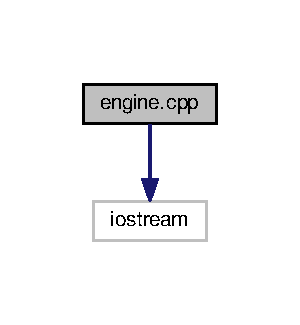
\includegraphics[width=144pt]{engine_8cpp__incl}
\end{center}
\end{figure}
\subsection*{Functions}
\begin{DoxyCompactItemize}
\item 
int \hyperlink{engine_8cpp_a0ddf1224851353fc92bfbff6f499fa97}{main} (int argc, char $\ast$argv\mbox{[}$\,$\mbox{]})
\end{DoxyCompactItemize}


\subsection{Function Documentation}
\hypertarget{engine_8cpp_a0ddf1224851353fc92bfbff6f499fa97}{\index{engine.\-cpp@{engine.\-cpp}!main@{main}}
\index{main@{main}!engine.cpp@{engine.\-cpp}}
\subsubsection[{main}]{\setlength{\rightskip}{0pt plus 5cm}int main (
\begin{DoxyParamCaption}
\item[{int}]{argc, }
\item[{char $\ast$}]{argv\mbox{[}$\,$\mbox{]}}
\end{DoxyParamCaption}
)}}\label{engine_8cpp_a0ddf1224851353fc92bfbff6f499fa97}


Definition at line 17 of file engine.\-cpp.


\hypertarget{README_8md}{\section{R\-E\-A\-D\-M\-E.\-md File Reference}
\label{README_8md}\index{R\-E\-A\-D\-M\-E.\-md@{R\-E\-A\-D\-M\-E.\-md}}
}

\hypertarget{version_8hpp}{\section{version.\-hpp File Reference}
\label{version_8hpp}\index{version.\-hpp@{version.\-hpp}}
}


Software Version Header.  


\subsection*{Macros}
\begin{DoxyCompactItemize}
\item 
\#define \hyperlink{version_8hpp_ad4471b132ffbd3c3ef43967b452eefce}{C\-O\-S\-S\-B\-\_\-\-V\-E\-R\-S\-I\-O\-N\-\_\-\-M\-A\-J\-O\-R}~0
\item 
\#define \hyperlink{version_8hpp_aae1d764abec9bab80a51a3c68fa13843}{C\-O\-S\-S\-B\-\_\-\-V\-E\-R\-S\-I\-O\-N\-\_\-\-M\-I\-N\-O\-R}~0
\item 
\#define \hyperlink{version_8hpp_a612899b5ecb63fedff55b5d5a0c08c18}{C\-O\-S\-S\-B\-\_\-\-V\-E\-R\-S\-I\-O\-N\-\_\-\-R\-E\-V}~1
\item 
\#define \hyperlink{version_8hpp_a69c5ca0c2d0c12361254d6620a359ea8}{V\-E\-R\-S\-I\-O\-N\-\_\-\-S\-T\-R}(x)~\#x
\item 
\#define \hyperlink{version_8hpp_a87a9e35ad5f563ae6010a151daa034a6}{C\-O\-S\-S\-B\-\_\-\-V\-E\-R\-S\-I\-O\-N\-\_\-\-S\-E\-T}(major, minor, rev)~\hyperlink{version_8hpp_a69c5ca0c2d0c12361254d6620a359ea8}{V\-E\-R\-S\-I\-O\-N\-\_\-\-S\-T\-R}(major) \char`\"{}.\char`\"{} \hyperlink{version_8hpp_a69c5ca0c2d0c12361254d6620a359ea8}{V\-E\-R\-S\-I\-O\-N\-\_\-\-S\-T\-R}(minor) \char`\"{}.\char`\"{} \hyperlink{version_8hpp_a69c5ca0c2d0c12361254d6620a359ea8}{V\-E\-R\-S\-I\-O\-N\-\_\-\-S\-T\-R}(rev)
\item 
\#define \hyperlink{version_8hpp_a19e84d161aab6f58beb44ff4b3b7082a}{C\-O\-S\-S\-B\-\_\-\-V\-E\-R\-S\-I\-O\-N}~\hyperlink{version_8hpp_a87a9e35ad5f563ae6010a151daa034a6}{C\-O\-S\-S\-B\-\_\-\-V\-E\-R\-S\-I\-O\-N\-\_\-\-S\-E\-T}(\hyperlink{version_8hpp_ad4471b132ffbd3c3ef43967b452eefce}{C\-O\-S\-S\-B\-\_\-\-V\-E\-R\-S\-I\-O\-N\-\_\-\-M\-A\-J\-O\-R}, \hyperlink{version_8hpp_aae1d764abec9bab80a51a3c68fa13843}{C\-O\-S\-S\-B\-\_\-\-V\-E\-R\-S\-I\-O\-N\-\_\-\-M\-I\-N\-O\-R}, \hyperlink{version_8hpp_a612899b5ecb63fedff55b5d5a0c08c18}{C\-O\-S\-S\-B\-\_\-\-V\-E\-R\-S\-I\-O\-N\-\_\-\-R\-E\-V})
\end{DoxyCompactItemize}


\subsection{Detailed Description}
Software Version Header. \begin{DoxyAuthor}{Author}
Byunghun Hwang\href{mailto:bhhwang@nsynapse.com}{\tt bhhwang@nsynapse.\-com} 
\end{DoxyAuthor}
\begin{DoxyDate}{Date}
2015. 6. 9 
\end{DoxyDate}


Definition in file \hyperlink{version_8hpp_source}{version.\-hpp}.



\subsection{Macro Definition Documentation}
\hypertarget{version_8hpp_a19e84d161aab6f58beb44ff4b3b7082a}{\index{version.\-hpp@{version.\-hpp}!C\-O\-S\-S\-B\-\_\-\-V\-E\-R\-S\-I\-O\-N@{C\-O\-S\-S\-B\-\_\-\-V\-E\-R\-S\-I\-O\-N}}
\index{C\-O\-S\-S\-B\-\_\-\-V\-E\-R\-S\-I\-O\-N@{C\-O\-S\-S\-B\-\_\-\-V\-E\-R\-S\-I\-O\-N}!version.hpp@{version.\-hpp}}
\subsubsection[{C\-O\-S\-S\-B\-\_\-\-V\-E\-R\-S\-I\-O\-N}]{\setlength{\rightskip}{0pt plus 5cm}\#define C\-O\-S\-S\-B\-\_\-\-V\-E\-R\-S\-I\-O\-N~{\bf C\-O\-S\-S\-B\-\_\-\-V\-E\-R\-S\-I\-O\-N\-\_\-\-S\-E\-T}({\bf C\-O\-S\-S\-B\-\_\-\-V\-E\-R\-S\-I\-O\-N\-\_\-\-M\-A\-J\-O\-R}, {\bf C\-O\-S\-S\-B\-\_\-\-V\-E\-R\-S\-I\-O\-N\-\_\-\-M\-I\-N\-O\-R}, {\bf C\-O\-S\-S\-B\-\_\-\-V\-E\-R\-S\-I\-O\-N\-\_\-\-R\-E\-V})}}\label{version_8hpp_a19e84d161aab6f58beb44ff4b3b7082a}


Definition at line 18 of file version.\-hpp.

\hypertarget{version_8hpp_ad4471b132ffbd3c3ef43967b452eefce}{\index{version.\-hpp@{version.\-hpp}!C\-O\-S\-S\-B\-\_\-\-V\-E\-R\-S\-I\-O\-N\-\_\-\-M\-A\-J\-O\-R@{C\-O\-S\-S\-B\-\_\-\-V\-E\-R\-S\-I\-O\-N\-\_\-\-M\-A\-J\-O\-R}}
\index{C\-O\-S\-S\-B\-\_\-\-V\-E\-R\-S\-I\-O\-N\-\_\-\-M\-A\-J\-O\-R@{C\-O\-S\-S\-B\-\_\-\-V\-E\-R\-S\-I\-O\-N\-\_\-\-M\-A\-J\-O\-R}!version.hpp@{version.\-hpp}}
\subsubsection[{C\-O\-S\-S\-B\-\_\-\-V\-E\-R\-S\-I\-O\-N\-\_\-\-M\-A\-J\-O\-R}]{\setlength{\rightskip}{0pt plus 5cm}\#define C\-O\-S\-S\-B\-\_\-\-V\-E\-R\-S\-I\-O\-N\-\_\-\-M\-A\-J\-O\-R~0}}\label{version_8hpp_ad4471b132ffbd3c3ef43967b452eefce}


Definition at line 12 of file version.\-hpp.

\hypertarget{version_8hpp_aae1d764abec9bab80a51a3c68fa13843}{\index{version.\-hpp@{version.\-hpp}!C\-O\-S\-S\-B\-\_\-\-V\-E\-R\-S\-I\-O\-N\-\_\-\-M\-I\-N\-O\-R@{C\-O\-S\-S\-B\-\_\-\-V\-E\-R\-S\-I\-O\-N\-\_\-\-M\-I\-N\-O\-R}}
\index{C\-O\-S\-S\-B\-\_\-\-V\-E\-R\-S\-I\-O\-N\-\_\-\-M\-I\-N\-O\-R@{C\-O\-S\-S\-B\-\_\-\-V\-E\-R\-S\-I\-O\-N\-\_\-\-M\-I\-N\-O\-R}!version.hpp@{version.\-hpp}}
\subsubsection[{C\-O\-S\-S\-B\-\_\-\-V\-E\-R\-S\-I\-O\-N\-\_\-\-M\-I\-N\-O\-R}]{\setlength{\rightskip}{0pt plus 5cm}\#define C\-O\-S\-S\-B\-\_\-\-V\-E\-R\-S\-I\-O\-N\-\_\-\-M\-I\-N\-O\-R~0}}\label{version_8hpp_aae1d764abec9bab80a51a3c68fa13843}


Definition at line 13 of file version.\-hpp.

\hypertarget{version_8hpp_a612899b5ecb63fedff55b5d5a0c08c18}{\index{version.\-hpp@{version.\-hpp}!C\-O\-S\-S\-B\-\_\-\-V\-E\-R\-S\-I\-O\-N\-\_\-\-R\-E\-V@{C\-O\-S\-S\-B\-\_\-\-V\-E\-R\-S\-I\-O\-N\-\_\-\-R\-E\-V}}
\index{C\-O\-S\-S\-B\-\_\-\-V\-E\-R\-S\-I\-O\-N\-\_\-\-R\-E\-V@{C\-O\-S\-S\-B\-\_\-\-V\-E\-R\-S\-I\-O\-N\-\_\-\-R\-E\-V}!version.hpp@{version.\-hpp}}
\subsubsection[{C\-O\-S\-S\-B\-\_\-\-V\-E\-R\-S\-I\-O\-N\-\_\-\-R\-E\-V}]{\setlength{\rightskip}{0pt plus 5cm}\#define C\-O\-S\-S\-B\-\_\-\-V\-E\-R\-S\-I\-O\-N\-\_\-\-R\-E\-V~1}}\label{version_8hpp_a612899b5ecb63fedff55b5d5a0c08c18}


Definition at line 14 of file version.\-hpp.

\hypertarget{version_8hpp_a87a9e35ad5f563ae6010a151daa034a6}{\index{version.\-hpp@{version.\-hpp}!C\-O\-S\-S\-B\-\_\-\-V\-E\-R\-S\-I\-O\-N\-\_\-\-S\-E\-T@{C\-O\-S\-S\-B\-\_\-\-V\-E\-R\-S\-I\-O\-N\-\_\-\-S\-E\-T}}
\index{C\-O\-S\-S\-B\-\_\-\-V\-E\-R\-S\-I\-O\-N\-\_\-\-S\-E\-T@{C\-O\-S\-S\-B\-\_\-\-V\-E\-R\-S\-I\-O\-N\-\_\-\-S\-E\-T}!version.hpp@{version.\-hpp}}
\subsubsection[{C\-O\-S\-S\-B\-\_\-\-V\-E\-R\-S\-I\-O\-N\-\_\-\-S\-E\-T}]{\setlength{\rightskip}{0pt plus 5cm}\#define C\-O\-S\-S\-B\-\_\-\-V\-E\-R\-S\-I\-O\-N\-\_\-\-S\-E\-T(
\begin{DoxyParamCaption}
\item[{}]{major, }
\item[{}]{minor, }
\item[{}]{rev}
\end{DoxyParamCaption}
)~{\bf V\-E\-R\-S\-I\-O\-N\-\_\-\-S\-T\-R}(major) \char`\"{}.\char`\"{} {\bf V\-E\-R\-S\-I\-O\-N\-\_\-\-S\-T\-R}(minor) \char`\"{}.\char`\"{} {\bf V\-E\-R\-S\-I\-O\-N\-\_\-\-S\-T\-R}(rev)}}\label{version_8hpp_a87a9e35ad5f563ae6010a151daa034a6}


Definition at line 17 of file version.\-hpp.

\hypertarget{version_8hpp_a69c5ca0c2d0c12361254d6620a359ea8}{\index{version.\-hpp@{version.\-hpp}!V\-E\-R\-S\-I\-O\-N\-\_\-\-S\-T\-R@{V\-E\-R\-S\-I\-O\-N\-\_\-\-S\-T\-R}}
\index{V\-E\-R\-S\-I\-O\-N\-\_\-\-S\-T\-R@{V\-E\-R\-S\-I\-O\-N\-\_\-\-S\-T\-R}!version.hpp@{version.\-hpp}}
\subsubsection[{V\-E\-R\-S\-I\-O\-N\-\_\-\-S\-T\-R}]{\setlength{\rightskip}{0pt plus 5cm}\#define V\-E\-R\-S\-I\-O\-N\-\_\-\-S\-T\-R(
\begin{DoxyParamCaption}
\item[{}]{x}
\end{DoxyParamCaption}
)~\#x}}\label{version_8hpp_a69c5ca0c2d0c12361254d6620a359ea8}


Definition at line 16 of file version.\-hpp.


%--- End generated contents ---

% Index
\newpage
\phantomsection
\addcontentsline{toc}{chapter}{Index}
\printindex

\end{document}
